\chapter{Productivity tools}
As we we begin the development of the Easy Web Content Site Builder from scratch, it gave us the opportunity to set-up a bunch of productivity tools. These tool are about automatize tasks, enhance code quality, debug, teamwork, documentation.
\section{Pear}

PEAR is a framework and distribution system for reusable PHP components. It allows to easily install, remove and update php libraries and packages by using simple command line.
\\

\lstset{language=bash}
\begin{lstlisting}[label=pear-install,caption=Installation of pear packages]
C:\...>pear channel-discover channelname
C:\...>pear install --alldeps channelname/packagename
\end{lstlisting}

\section{Phing}

To work more efficently automatic build task could be used to improve productivity. Phing is a tool written in PHP. It is very similar to famous ANT.
Phing is a build tool. A phing build task has been set to automatize js/css minification with YUI Compress.
Right now we can use it to automate deployment and development.
\begin{itemize}
\item automatic js / css minify for release
\item automatic backup
\item automatic database deployment
\item generate php documentaion from comments
\end{itemize}

Phing uses pear to be installed automatically.

\lstset{language=bash}
\begin{lstlisting}[label=phing-install,caption=Installation of Phing]
C:\...>pear channel-discover channelname
C:\...>pear install --alldeps channelname/packagename
\end{lstlisting}

A build is configured with an xml file : build.xml. It allows to program automated tasks called targets. Target can be combined and ordered.
Obfuscate javascript or css file would have been a very repetitive and boring task to do manually. This tool allows to keep code unobfuscated for development environement (easy to debug and read), and obfuscated in production environment (lighter, faster and harder to read).

\lstset{language=Ant}
\begin{lstlisting}[label=phing-build,caption=Example of Phing build.xml]
<project name="EasyWebSite" basedir="." default="info">
	<property name="ProjectVersion" value="0.0.1" />
	<target name="minify-js">
		<minify targetDir="${releaseDirectory}/Framework/public/js/"
				yuiPath="${buildScriptsDirectory}/yuicompressor-2.4.2.jar">
			<fileset dir="${applicationDirectory}/Framework/public/js/">
			<include name="**/*.js"/>
			<exclude name="library/**"/>
			</fileset>
		</minify>
	</target>	
	<target name="zip-backup"
		description="Creates a backup of the project">
		<echo msg="Backup to zip archive"/>
		<copy file="build.xml" tofile="build.xml.backup" overwrite="true"/>
		<mkdir dir="${backupDirectory}" />				
		<zip destfile="${backupDirectory}/ews_backup-${ProjectDate}.zip">
		<fileset dir=".">
			<include name="build.xml" />
			<exclude name="build/**"/>
			<exclude name="docs/**"/>
			<include name="src/**" />			
		</fileset>
		</zip>
	</target>
	<target name="build-all" depends="cleanup , setup-environments, prepare-libs , execute-phpdoc, execute-jsdoc , deploying-debug, deploying-release, minify-js ,minify-css, deploy-database"
		description="deploys full environment">       
		<echo msg="Fin du build" />		
	</target>		
</project>
\end{lstlisting}



\section{Subversion}

Subversion is a version control system. It allows to keep track to modifications of files revision after revision. A system like this is very important to use in a team environment. For several reasons.

\paragraph*{Critic portions of code}
When working on important pieces of code the developer is often afraid to introduce bugs of to make the application crash. With a version control system, he can rollback to previous stable version of the code easily. So he can experiment new features with more confidence. 

\paragraph*{Debug}
If a bug is introduced, the developer can check what were the modifications in which files by using a diff tool to compare two revisions of a the same file.

\begin{figure}[!ht]
\centering
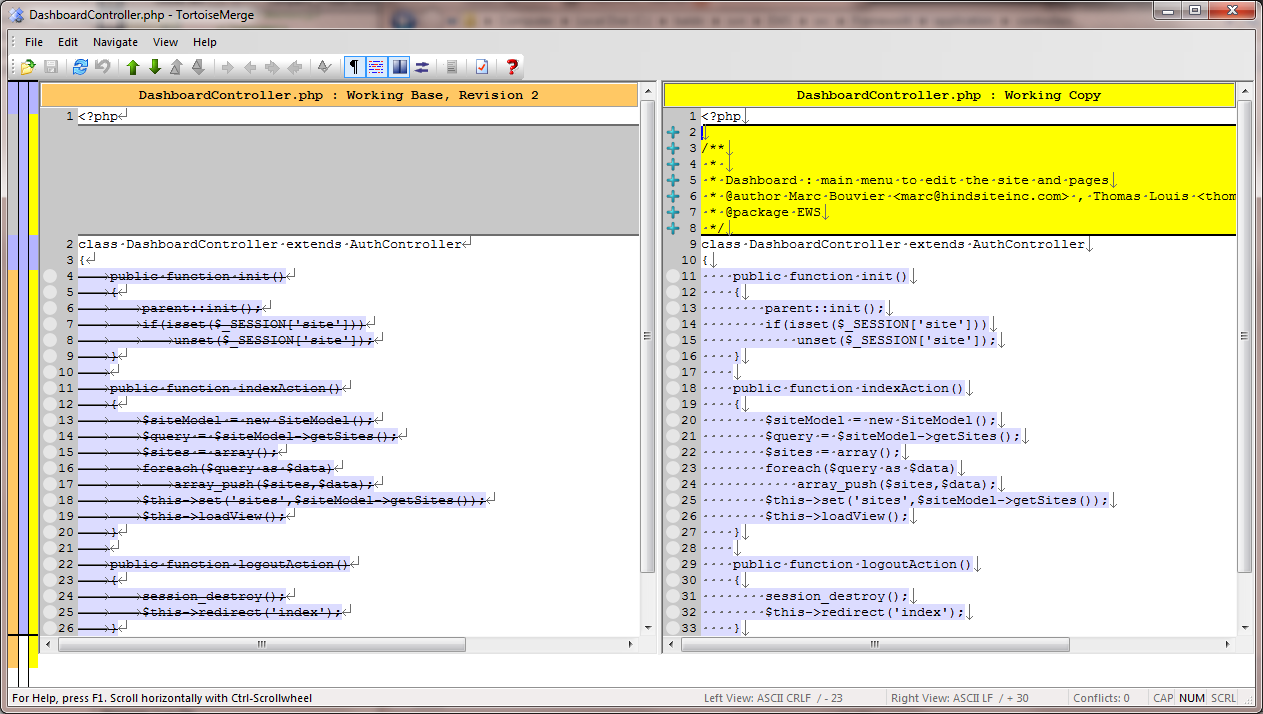
\includegraphics[width=.85\textwidth]{img/diff.png}
\caption{Diff tool}
\label{figure:diff}
\end{figure}

- compare sources between different revisions
- team work work on the very same files / not overwrites someone elses modifications

\section{Code documentation}

\subsection{PHPDoc}

\subsection{JSDoc}


\section{Netbeans}
-code autocompletion
- code navigation
- code syntax recognition
- classes heritage detection

\section{Mantis}
We used 

